\documentclass[a4paper, 12pt]{report}  % set doc type and font size
\usepackage{fontspec}
\usepackage[left=2cm,right=2cm,top=2.2cm,bottom=2.2cm]{geometry}

% math tools
\usepackage{amsmath}
\usepackage{amssymb}
\usepackage{amsfonts}

\usepackage{makecell}

\usepackage[most]{tcolorbox}
\usepackage{xcolor}
\newtcolorbox{codeblock}{
  enhanced,
  breakable,
  colback=gray!5,
  colframe=black,
  boxrule=0.5pt,
  arc=2pt,
  left=6pt,
  right=6pt,
  top=6pt,
  bottom=6pt
}

\setlength{\parindent}{0pt}
\setlength{\parskip}{0.45em}
\usepackage{enumitem}

% figures and tables
\usepackage{graphicx}
\usepackage{float}
\usepackage{booktabs}
\usepackage{tikz}
\usetikzlibrary{arrows.meta, positioning, shapes.geometric}
\graphicspath{{../outputs/}}

% chapter title format
\newcommand{\zhnum}[1]{%
  \ifcase#1\or 一\or 二\or 三\or 四\or 五\or 六\or 七\or 八\or 九\or 十\else #1\fi}
\renewcommand{\thechapter}{第\zhnum{\value{chapter}}章}
\makeatletter
\def\@makechapterhead#1{%
  \vspace*{0.5em}%
  {\parindent \z@ \raggedright \normalfont
    \huge\bfseries \thechapter\quad #1\par\nobreak
    \vskip 1.2em
  }}
\def\@makeschapterhead#1{%
  \vspace*{0.5em}%
  {\parindent \z@ \raggedright \normalfont
    \huge\bfseries #1\par\nobreak
    \vskip 1.2em
  }}
\makeatother
% change "table" to "表"
\renewcommand{\tablename}{表}
\counterwithout{table}{chapter}
% change "figur" to "圖"
\renewcommand{\figurename}{圖}
\counterwithout{figure}{chapter}

% set chinese
\usepackage{xeCJK}
\xeCJKsetup{AutoFakeBold=true, AutoFakeSlant=true}
\setmainfont{Times New Roman}
\setCJKmainfont{標楷體}

\title{\textbf{半導體製程資料之統計製程監控分析}}
\author{黃丞暘 \quad 611211106\\統計專論 (III) 期末報告（修訂）}
\date{2026 年 6 月 16 日}

\begin{document}
\maketitle

\chapter{目的}

針對 SEmi-COnductor manufacturing (SECOM) 半導體製程資料建立一套完整的第一階段（以下稱 Phase I）及第二階段監控（以下稱 Phase II）統計製程監控流程。
分析流程包含：

\begin{enumerate}[label=(\arabic*)]
  \item 選擇一個可用的變數
  \item 依 \(m=\lfloor 0.5n \rfloor\) 將資料分為 Phase I 與 Phase II
  \item 移除 Phase I 的缺失值與離群值（3倍IQR）
  \item 於 Phase I 使用 RS/P 方法檢查是否有水準偏移（level shift）或尺度偏移（scale shift）
  \item 於 Phase II 建立 Shewhart、EWMA、CUSUM 與 CPD 管制圖
  \item 比較各方法第一次出現訊號的時間（first signal）與發出訊號的總次數（signal counts）
  \item 解釋製程型態較可能為平均數偏移（mean shift）、變異數偏移（variance shift）或結構性改變（structural change）
\end{enumerate}

核心問題是哪一張管制圖最早發出訊號（signal）？
這個訊號比較像是平均數偏移、變異數偏移，還是結構性改變？

\chapter{資料介紹}

\section*{資料來源}

使用 UCI 的 SECOM。
資料共有 1567 筆樣本與 590 個變數。
另外，
包含時間欄位與 Pass/Fail 的標記。

\section*{變數選擇}

選用的變數為 \(x_{297}\)，
理由是：

\begin{itemize}
  \item 缺失比例低，只有 2 筆缺失值
  \item 有足夠多的相異數值，且不屬於常數欄位
\end{itemize}

\chapter{建立 Phase I}

\section*{切分}

令
\[
  m=\lfloor 0.5n \rfloor
\]
原始資料共有 \(n=1567\) 筆，因此
\[
  m=\lfloor 0.5(1567) \rfloor = 783
\]
前 783 筆樣本作為 Phase I 的參考資料，
後 784 筆樣本作為 Phase II 的監控資料。

圖 \ref{fig:series} 顯示資料的排序與 Phase I/II 的分界位置。

\begin{figure}[H]
  \centering
  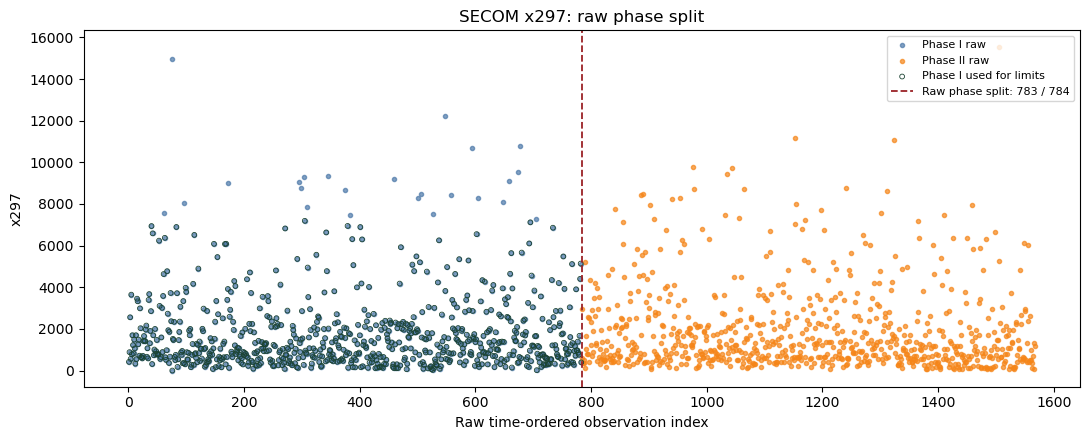
\includegraphics[width=0.95\linewidth]{series_phase_split2.png}
  \caption{Phase I/II 分界位置}
  \label{fig:series}
\end{figure}

\section*{Phase I 資料前處理}

先刪除 \(x_{297}\) 的缺失值，
再使用 $3 IQR$ 的規則刪除離群值。
若樣本低於 \(Q_1-3IQR=-4376.27\) 或高於 \(Q_3+3IQR=7265.77\)，
則視為離群值並刪除。
如表 \ref{tab:preprocessing} 所示，
清理後的樣本為 757 筆。

\begin{table}[H]
  \centering
  \caption{資料前處理摘要}
  \label{tab:preprocessing}
  \vspace{0.5em}
  \begin{tabular}{|l|r|}
    \hline
     & 筆數 \\
    \hline
    原始樣本數 & 783 \\
    移除缺失值數 & 2 \\
    移除 3 倍 IQR 離群值數 & 24 \\
    \hline
    清理後樣本數 & 757 \\
    \hline
  \end{tabular}
\end{table}

\begin{figure}[H]
  \centering
  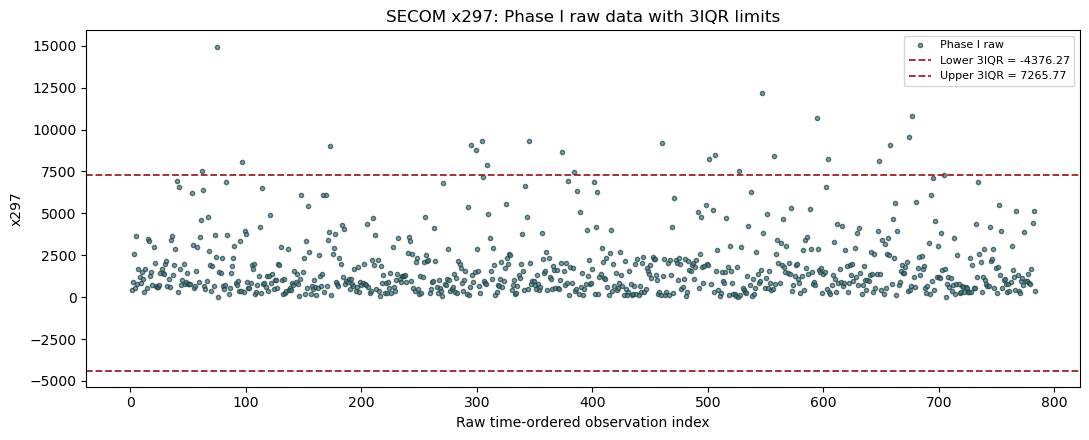
\includegraphics[width=0.95\linewidth]{series_phaseIraw.png}
  \caption{在 3 倍 IQR 下的 Phase I 散佈圖}
  \label{fig:Iraw}
\end{figure}

\section*{敘述統計}

在 Phase I 清理後的敘述統計如表 \ref{tab:summary} 所示。
此變數具有相當大的變異程度，
且平均數高於中位數，
由圖 \ref{fig:Icleaned} 可知，
顯示資料分佈為右偏態，
不符合常態分佈。

\begin{table}[H]
  \centering
  \caption{清理後 Phase I 敘述統計}
  \vspace{0.5em}
  \label{tab:summary}
  \begin{tabular}{|l|r|r|r|r|r|r|r|}
    \hline
    平均數 & 標準差 & 最小值 & Q1 & 中位數 & Q3 & 最大值 \\
    \hline
    1629.34 & 1478.01 & 0.00 & 598.12 & 1141.48 & 2109.16 & 7189.73 \\
    \hline
  \end{tabular}
\end{table}

\begin{figure}[H]
  \centering
  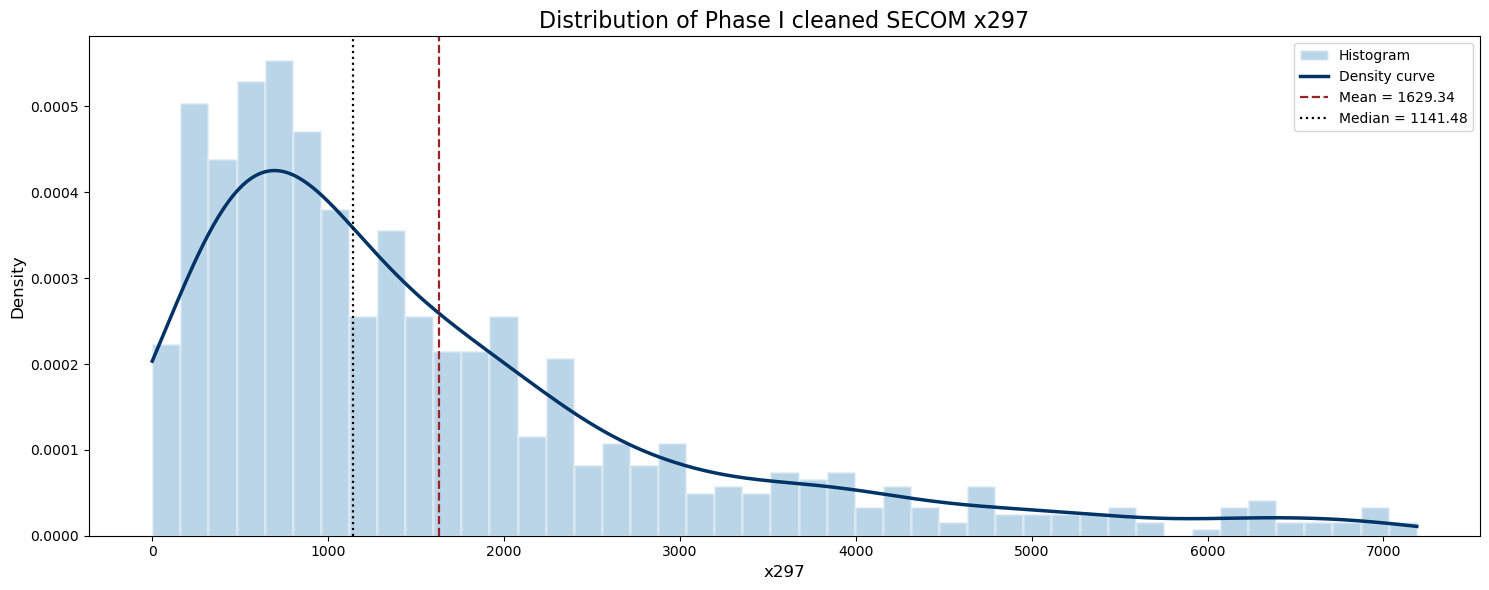
\includegraphics[width=0.95\linewidth]{variable_distribution_x297_phaseI.png}
  \caption{前處理完 Phase I 分佈}
  \label{fig:Icleaned}
\end{figure}

\section*{Phase I RS/P 穩定性診斷}

Phase I 的目的在於建立管制界線內的參考樣本，
因此必須先檢查 Phase I 是否具有明顯的水準偏移或尺度偏移。
使用遞迴分割（Recursive Segmentation, 以下稱 RS）及置換校準（Permutation Calibration, 以下稱 P） 的方法進行診斷。
分別以 $p_{\text{level}}$ 、 $p_{\text{scale}}$ 與 $0.05$ 的關係來確認 Phase I 的資料是否穩定，若小於，則不穩定，反之，則穩定。其診斷結果如下：

\[
  p_{\text{level}} = 0.9650,\qquad
  p_{\text{scale}} = 0.7450
\]

兩個 p-value 皆遠大於 0.05，
因此沒有足夠證據拒絕 Phase I 的水準或尺度是穩定的假設。
也就是說，
Phase I 可視為合理的參考樣本，
可視為穩定的製程狀態，
如圖 \ref{fig:phIRSP} 所示。

\begin{figure}[H]
  \centering
  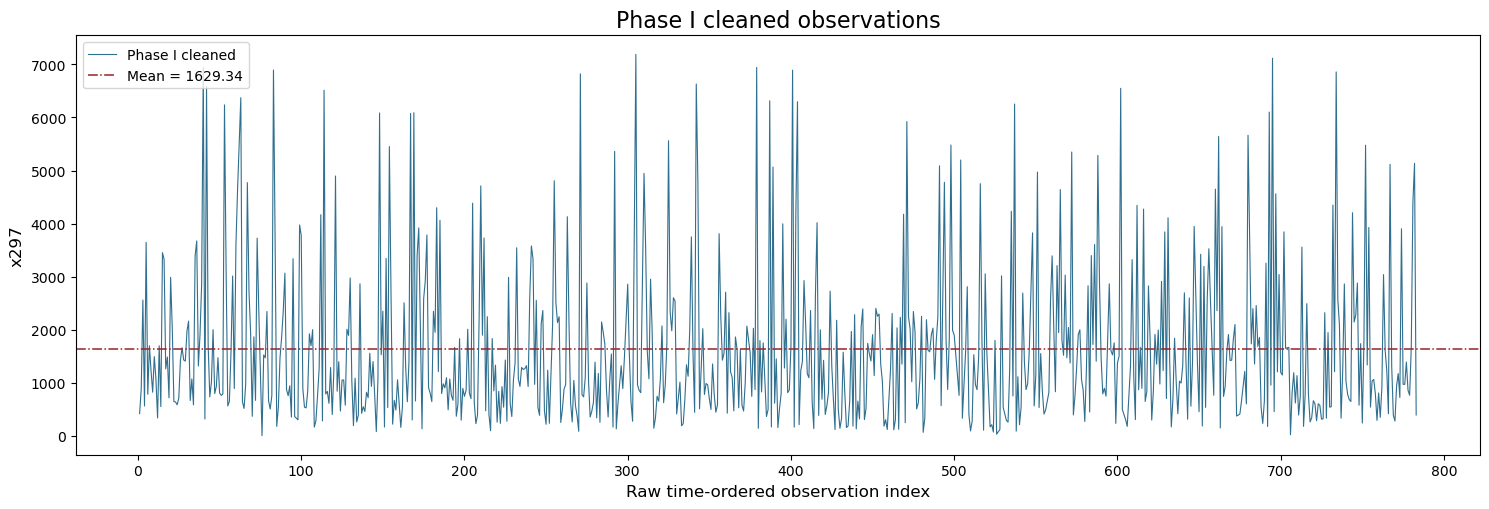
\includegraphics[width=0.95\linewidth]{series_phaseIrawRSP.png}
  \caption{Phase I RS/P}
  \label{fig:phIRSP}
\end{figure}

\chapter{監控 Phase II}

\section*{Gamma Individuals Shewhart chart}

考量 \(x_{297}\) 的資料屬於非負值且右偏態，
因此以 Phase I 清理後資料適合 Gamma 分配，
並建立 Individuals Shewhart chart。
下管制界線設定為 0，
上管制界線則由 Gamma 分配的上尾分位數決定。

表 \ref{tab:gammasetting} 結果顯示，
Phase II 第一次超過 Gamma 上管制界線的位置為原始樣本編號 842，
整段 Phase II 共有 23 筆樣本超過上管制界線。
此結果表示 Phase II 中存在若干單點極端高值，
但這並不必然代表整段 Phase II 發生持續性的水準偏移或尺度偏移。

\begin{table}[H]
  \centering
  \caption{Gamma Individuals Shewhart 管制界線摘要}
  \vspace{0.5em}
  \label{tab:gammasetting}
  \begin{tabular}{|l|r|}
    \hline
    參數 & 數值 \\
    \hline
    $\alpha$ & 1.36 \\
    \hline
    $\theta$ & 1199.01 \\
    \hline
    上管制界線 UCL & 7338.84 \\
    \hline
    下管制界線 LCL & 0 \\
    \hline
    Phase II 超過 UCL 筆數 & 23 \\
    \hline
    Phase II 第一個超過 UCL 的原始 index & 842 \\
    \hline
  \end{tabular}
\end{table}

\begin{figure}[H]
  \centering
  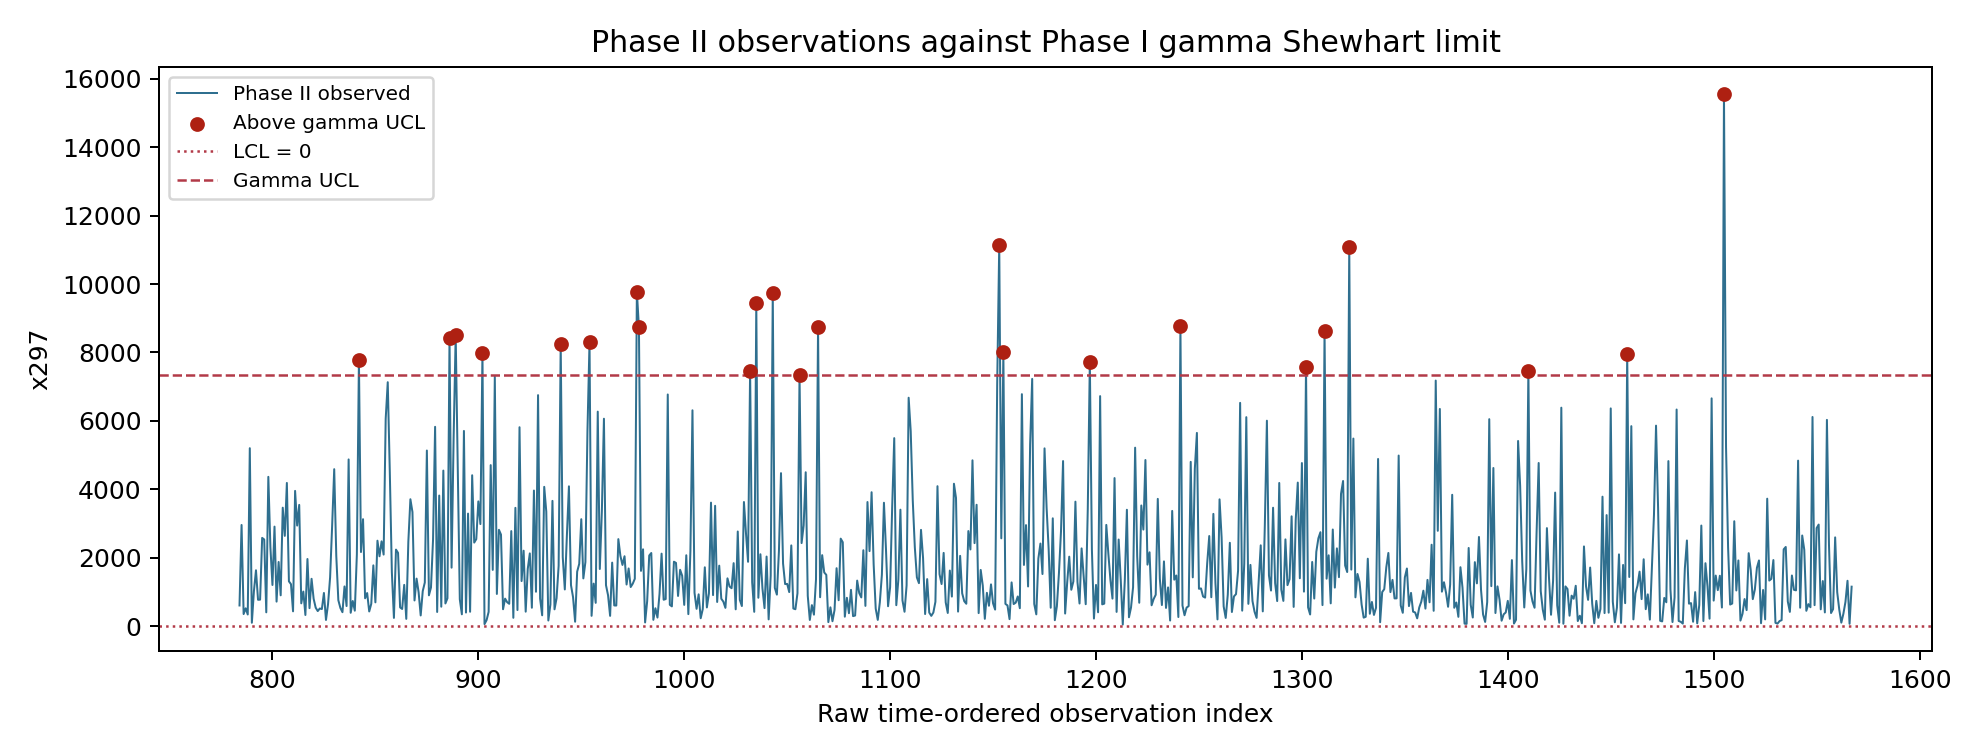
\includegraphics[width=0.85\linewidth]{phaseii_gamma_shewhart.png}
  \caption{Gamma Shewhart 管制界線下的 Phase II}
  \label{fig:gammaresult}
\end{figure}

\section*{Phase II RS/P 穩定性診斷}

由於 Phase I 資料分佈呈現明顯偏態，
若直接使用以常態分配為基礎設計的 EWMA、CUSUM 與 CPD 管制圖，
可能會使管制界線與發現訊號受到分配假設不符的影響。
因此，
改採用無母數的 RS/P 方法，
對 Phase II 資料進行結構穩定性診斷，
進一步對整段 Phase II 資料使用 RS/P 方法進行水準偏移或尺度偏移。

在 0.05 顯著水準下，
整段 Phase II 的 level 與 scale 診斷結果皆未達顯著。
其中，
$p_{level}=0.0575$，
雖然接近 0.05，
但仍未低於顯著水準，
因此尚不足以判定 Phase II 存在顯著的水準偏移。

水準與尺度偏移的估計切點皆落在 Phase II 末段，
對應樣本編號 1559。
由於該位置已接近整個製程觀測期間的結尾，
即使此處存在些微變化，
其後續可用於確認結構改變的資料量也相當有限。
因此不再進一步切割 Phase II 資料，
並判定整段 Phase II 製程未出現明顯的結構性改變。

\begin{table}[H]
  \centering
  \caption{Phase II RS/P 診斷}
  \label{tab:phaseIIrsp}
  \vspace{0.5em}
  \begin{tabular}{|l|r|r|r|r|}
    \hline
     & p-value & Phase II 估計切點 & 樣本編號 \\
    \hline
    Level & 0.0575 & 776 & 1559 \\
    \hline
    Scale & 0.1000 & 776 & 1559 \\
    \hline
  \end{tabular}
\end{table}

\begin{figure}[H]
  \centering
  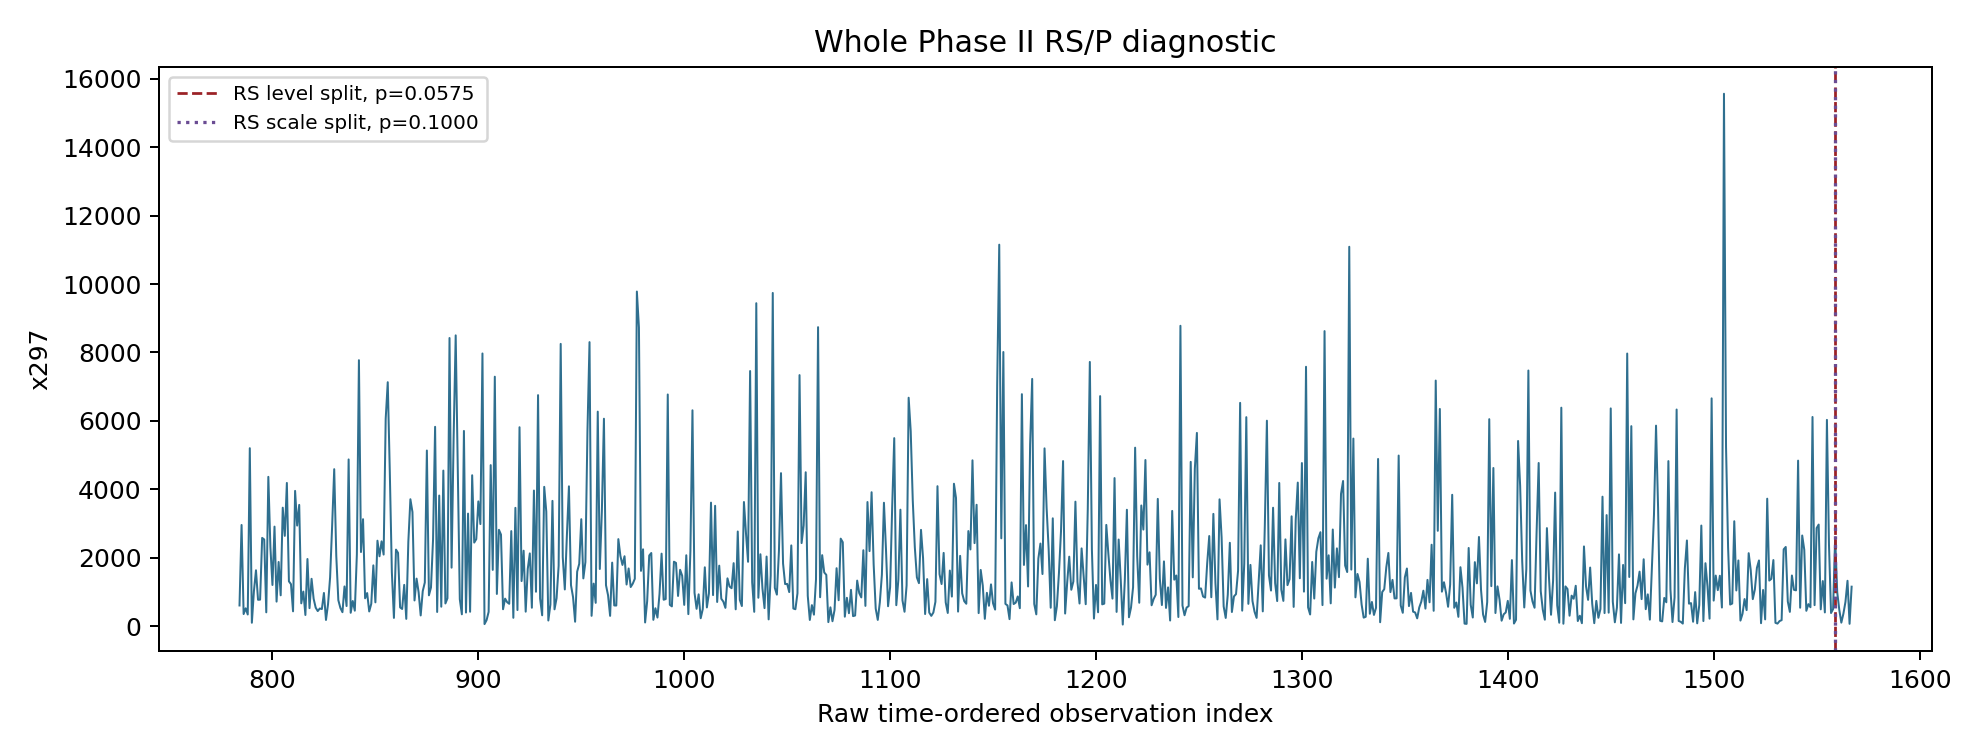
\includegraphics[width=0.85\linewidth]{phaseii_rsp_diagnosis.png}
  \label{fig:phaseIIrsp}
  \caption{Phase II 觀測值與 Gamma Shewhart 上管制界線}
\end{figure}

\chapter{結論}

針對 SECOM 資料中的 \(x_{297}\) 變數建立完整的 Phase I/II SPC 分析流程。
原始資料共有 1567 筆樣本，
依時間順序以前一半資料作為 Phase I，
後一半資料作為 Phase II。
因此，
前 783 筆樣本作為 Phase I 的參考資料，
後 784 筆樣本作為 Phase II 的監控資料。
其中，
Phase I 的 RS/P 診斷顯示 Phase I 沒有明顯 level 或 scale 不穩定，
可作為監控的參考。

由 Phase I 清理後的分佈可知，
\(x_{297}\) 呈現明顯右偏態，
且資料為非負值。
因此，
本研究不採用以常態分配為基礎的 3-sigma Shewhart、EWMA、CUSUM 與 CPD 管制圖，
而是使用 Gamma 分配建立 Individuals Shewhart chart 以及 RS/P 方法進行穩定性診斷。
結果顯示 Phase II 的 level 與 scale 診斷在 0.05 顯著水準下皆未達顯著；
level 與 scale 的估計切點皆落在 Phase II 末段，
由於該位置接近監控期間末段，
後續的資料量有限，
因此不再將 Phase II 切割為多個區段。
綜合上述，
目前無足夠證據顯示 Phase II 發生顯著的製程結構改變。

\end{document}
